\documentclass[a4paper,smallheadings,11pt,oneside,bibliography=totoc]{scrreprt}
\addtokomafont{disposition}{\rmfamily}
\usepackage[utf8x]{inputenc}
\usepackage[english]{babel}
\usepackage{amssymb}
\usepackage{amsthm}
\usepackage{amsmath}
\usepackage[dvipsnames]{xcolor}
\usepackage{graphicx}
\usepackage{microtype}
\usepackage{palatino}
\usepackage[round,colon]{natbib}
\usepackage[hidelinks]{hyperref}
\usepackage[titletoc]{appendix}
\usepackage{pgfplots}
\pagestyle{headings}
\usepackage{parskip}
\usepackage{tikz-uml}
\usepackage{tikz}
\usepackage{tcolorbox}
\usepackage{longtable}
\tcbuselibrary{listings,skins}
\usetikzlibrary{calc}
\usetikzlibrary{arrows.meta}
\usetikzlibrary{chains}
\usepackage{epstopdf}
\usepackage{colortbl}
\usepackage{hhline}
\usepackage{wrapfig}
\usepackage[font=footnotesize,labelfont=bf]{caption}
\newcommand{\comments}[1]{\textcolor{OliveGreen}{[\emph{#1}]}}

\graphicspath{{images/}}
\newcommand{\cisco}{cisco_images}
\newcommand{\ciscoImageScale}{0.7}

\setcounter{secnumdepth}{3} 
\setcounter{tocdepth}{3}

% Custom fonts
\newenvironment{console_font}{\fontfamily{pcr}\selectfont}{\par}
\newcommand*{\code}{\ttfamily\selectfont}

\definecolor{codegreen}{rgb}{0,0.6,0}
\definecolor{codegray}{rgb}{0.5,0.5,0.5}
\definecolor{codepurple}{rgb}{0.58,0,0.82}
\definecolor{backcolour}{rgb}{0.95,0.95,0.92}

\newcommand{\Fail}{\cellcolor{red!15} Fail}
\newcommand{\Pass}{\cellcolor{green!15} Pass}
\newcommand{\header}[1]{\cellcolor{blue!10} #1 & \cellcolor{blue!10} & \cellcolor{blue!10} \\ \lineend}
\newcommand{\lineend}{\hhline{|-|-|-|}}
 
\lstdefinestyle{mystyle}{
    commentstyle=\color{codegreen},
    keywordstyle={\bf \color{blue}},
    numberstyle=\tiny\color{codegray},
    stringstyle=\color{codepurple},
    basicstyle=\footnotesize\ttfamily,
    breakatwhitespace=false,         
    breaklines=true,                 
    captionpos=b,                    
    keepspaces=true,                 
    numbers=left, 
    columns=fixed,                                   
    showspaces=false,                
    showstringspaces=false,
    showtabs=false,                  
    tabsize=7,
    language=Python,
    numberstyle=\tiny, 
	numbersep=8pt
}

%Used to format code listings
\newtcblisting{Code}[2][]{
	top=0cm,
	bottom=0cm,
	left=0.5cm,
	right=0cm,
	colback=white,
	colframe=black,
    arc=1pt, outer arc=1pt,
    listing only, 
    listing style=mystyle,
    title= ,
    #1
}

\newtcblisting{Scripts}[2][]{
	top=0cm,
	bottom=0cm,
	left=0.5cm,
	right=0cm,
	colback=white,
	colframe=black,
    arc=1pt, outer arc=1pt,
    listing only, 
    listing style={mystyle, language= },
    title=,
    #1
}

\newcommand{\width}{3cm}
\tikzset{%
	>={Latex[width=2mm,length=2mm]},
	% Specifications for style of nodes:
            base/.style = {draw=black,
                           minimum width=\width, 
                           text width=\width, 
                           minimum height=1cm, 
                           text centered},                           
            decision/.style = {base, diamond, fill=yellow!15, draw=red},
            normal/.style = {base, rectangle, rounded corners}}
            
\newcommand{\yesLink}[1]{--node[fill=white]{Yes}(#1)}
\newcommand{\noLink}[1]{--node[fill=white]{No}(#1)}

\begin{document}

	%Title Page
	\title{Compromised and Degraded Network Simulation}
	\newcommand{\reporttype}{Final Report}
	\newcommand{\degreetitle}{BSc}
	\newcommand{\progname}{Computer Science}
	\author{Aidan Fray}
	\newcommand{\wordcount}{13697}

	% Document format
	\makeatletter
\begin{titlepage}

\vspace*{-5em}
~~

\vfill

\begin{center}
{\huge \textbf{\@title}}\\
\vspace*{1em}
{\LARGE \textbf{\reporttype{}}}\\
\vspace*{2em}
{\Large Submitted for the \degreetitle{} in}\\
\vspace*{0.5em}
{\Large \progname{}}\\
\vspace*{2em}
{\Large \today}\\
\vspace*{2em}
{\Large by}\\
\vspace*{2em}
{\Large \textbf{\@author}}\\
\vspace*{3em}
{\large Word Count: \wordcount{}}
\end{center}

\vfill
\begin{center}
	\includegraphics[height=0.075\textheight]{title_page/UoH_Logo.pdf}
\end{center}

\end{titlepage}
\makeatother		
	\newpage
	\tableofcontents
	\chapter{Introduction}
Networks and their functionality play a crucial role in today's internet infrastructure. Networks relay packets and allow communication between computers from opposite sides of the globe. This paper will discuss and explore the effects of degradation on a live network, and how these effects can be reduced or negated. 

The live network will be a simulation of network traffic, this traffic will be routed through a custom router running on a small Raspberry Pi. This Raspberry Pi will run the degradation tool that will allow the control of network conditions. 

Issues may arise from various aspects of the project. The first issue being the accuracy in simulation of network traffic may cause inaccuracies in the tools validity. More problems may occur regrading the discovery of effective practises to negate hostile network conditions, and other issues involving the stability and scalability of the tool meaning its max capacity needs defining. These issues will be discussed later.

	\chapter{Aim and Objectives}

\comments{This section should define the overall aim of the project and clearly state the individual, measurable objectives that you have set for the project (objectives should have a deliverable outcome associated with them). In short, this section should clearly identify exactly what it is that you are intending to achieve in the project.}


State the overall aim of your project here. This can carry over on to several lines if you want.

Some text here to indicate that the above aim will be met by the following numbered objectives. Write approximately one sentence to outline what the objective is here. Include as many objectives as you think reasonable but remember that these are not as fine grained as the tasks which will come later.

\paragraph{Objective Title Goes Here If You Can Think Of One.} 
Here you should be writing a more detailed description of what this objective is. It should explain how it contributes towards the aim, what the deliverable(s) of the objective is/are, and how you intend to evaluate it.

\paragraph{Objective Title Goes Here If You Can Think Of One.} 
Do this for each one of your objectives.
	\chapter{Background}

\comments{This is a narrative description of the general context within which your project fits. Depending on your particular project characteristics, you are required to include discussion of any or all of the following – previous related work; the work or objectives of a client; the essential principles of systems or techniques you are using.
All this narrative should be properly referenced to source material citations. Remember that a high class project will refer to background sources beyond just those on the Web. 
In writing this section you should pay close attention to your audience and their prior knowledge of the subject(s) that you are discussing. You should assume that your reader is a student who has just completed the second year of your degree programme and can therefore assume that the reader is familiar with all topics taught up to the end of the second year. Anything that is needed to understand your project and its context but which has not been taught by the end of the second year of your degree should be discussed in this background section. 
This section may include one or more of the following subsections. It is difficult to give prescriptive guidance on which subsections you should include as this depends on the nature of the project you are undertaking – you should discuss this with your supervisor.}

\comments{
\textbf{Problem Context:}
If your project involves significant work on a non-computing topic that is likely to be unfamiliar to most readers (e.g. linguistics, fluid dynamics) you should describe the important principles, concepts and terminology of that subject area in some detail. You will have had to learn these yourself in getting to grips with this unfamiliar topic and you should summarize what you learnt to enable the reader to understand your subsequent discussion on your project work and how this relates to the wider topic area.}

\comments{
\textbf{Comparison of Technologies:}
If there are several possible technologies that could be used in your project work you should present a comparative analysis and critical appraisal of each of these technologies. You should create a subsection for each of the technologies you discuss and title each subsection with the name of the technology it describes (e.g. object-oriented databases, XML ). Within each subsection you should provide an overview of the technology, its key features and its strengths and weaknesses in relation to your project.}

\comments{
\textbf{Alternative Solutions:}
If others have produced solutions or addressed similar problems to those addressed by your project you should describe those alternative solutions here. Similarly, if several possible approaches suggest themselves as ways of solving the problems inherent in your project you should discuss those here. You should provide a comparative analysis and critical appraisal of each alternative solution approach or existing solution, identifying their key features and their strengths and weaknesses in relation to your project.}

\comments{
\textbf{Comparison of Algorithms:}
There may be a number of different algorithms which could be applied to the central problems in your project and you have had to choose which of these algorithms are the most appropriate for your implementation. If this is the case then you should provide a comparative analysis and critical appraisal of each of the potentially applicable algorithms, highlighting their key features and their strengths and weaknesses in relation to your project.
}

\comments{
\textbf{Processes and Methodology:}
If your project is concerned with improving, implementing or evaluating a particular technical process or method of working you should discuss these in detail. We are not expecting you to describe what software development methodology you are following in implementing your project and you certainly do not need to regurgitate textbook descriptions of the Waterfall method here as everyone already knows that model well.
}

\comments{
\textbf{Referencing:}
The current template provides a Bibtex style file (\texttt{hull.bst}) that conforms to the University's requirements of using Harvard referencing style \citep{Hull2016HarvardRef}. Your references should be collected as Bibtex entries into the file \texttt{report.bib}. Below are some examples of citing these Bibtex entries:
\begin{itemize}
\item \citet{Kazhdan2006} developed a technique for creating watertight surfaces from oriented point samples acquired with 3D range scanners.
\item Thorough coverage of the new C++11 standard can be found in \citep{Stroustrup2013}.
\item Vulkan is a cross-platform 3D graphics and compute API \citep{Vulkan2016}.
\item \citet{Canny1986} proposed a computational approach to detecting edges in images.
\end{itemize}
Many online digital libraries, such as those from ACM\footnote{\url{http://dl.acm.org/}} and IEEE\footnote{\url{http://ieeexplore.ieee.org/}}, provide Bibtex data for their papers. Google Scholar\footnote{\url{https://scholar.google.com}} is also an easy way to search for academic publications and their Bibtex data.
}
	%In this section you will discuss the Technical Development related to your project.
%In one or more chapters you must describe fully the design and development strategies you have adopted and the results achieved.  You may refer to appropriate User and System documentation presented as appendices to avoid repeating extensive detail, so you can focus here instead on a discussion of your reasons for adopting the techniques and strategies you have followed.

%Again, it is difficult to give prescriptive guidance on the subsection structure you might adopt, as this will depend on the nature and content of your project.  However, you will probably want at least to consider sections addressing issues of System Design; Implementation; Testing.  If there is a lot to cover in any of these areas, it may warrant presentation as a full chapter rather than a section.

\chapter{Technical Development}

% Section Description:
%
\section{Tool Architecture}
Below is the system architecture for the degradation tool:

\begin{center}
	\newcommand{\width}{3cm}
\newcommand{\imageScale}{0.2}

\tikzset{%
  >={Latex[width=2mm,length=2mm]},
  % Specifications for style of nodes:
            base/.style = {rectangle, rounded corners, draw=black,
                           minimum width=\width, minimum height=1cm,
                           text centered, font=\sffamily},
            red/.style = {base, fill=red!15},
            blue/.style = {base, fill=blue!15}}
          

\begin{center}
\begin{tikzpicture}[node distance=1.5cm, every node/.style={fill=white, font=\sffamily}, align=center]

	\node(User)[xshift=-10cm]{\includegraphics[scale=\imageScale]{User}};		
	\node(UserText)[below of=User]{User};		
	
	\node(GUI)[base, right of=User, xshift=(\width), yshift=2cm]{\includegraphics[scale=\imageScale]{Packet_UI_Design}};
	\node(GUIText)[below of=GUI, yshift=-0.5cm]{GUI};	
	
	\node(CLI)[base, below of=GUI, yshift=-2.25cm]{\includegraphics[scale=\imageScale]{CLI}};
	\node(CLIText)[below of=CLI]{CLI};
	
	\node(Effect)[blue, right of=User, xshift=(\width * 2) + 2cm]{Effect Choice};	
	\node(Nfqueue)[base, right of=Effect, xshift=(\width)]{NFQUEUE Creation};	
	
	\node(Parameters)[base, below of=Effect]{Parameter Handling};	
		
	
	\node(Packet)[red, below of=User, xshift=2cm, yshift=-4cm, text width=6cm]{Incomming Packets pushed into the NFQUEUE};
	\node(ChosenEffect)[blue, right of=Packet, xshift=\width + 2cm]{Chosen Effect};
	\node(PacketDescription)[above of=Packet, yshift=-0.5cm]{{\bf While NFQUEUE is running}};
	
	\draw[->] (User)--(GUI);
	\draw[->] (User)--(CLI);
	
	\draw[->] (GUI)--(Effect);
	\draw[->] (CLI)--(Parameters);
	\draw[->] (Parameters)--(Effect);	
	
	\draw[->] (Effect)--(Nfqueue);
	\draw[->] (Packet)--(ChosenEffect);
		
\end{tikzpicture}
\end{center}
	\begin{figure}[h]
		\caption{Architecture of the overall degradation tool}
	\end{figure}
\end{center}

It was decided early on that the script was to be controlled by two forms of interfaces; Graphical User Interface (GUI) and a text based Command Line Interface (CLI). This was to allow the tool to be run on the router (CLI) and also run on separate machines (GUI or CLI), this makes the tool versatile to many situations.

The system design is split into two stages:

\begin{itemize}
\item {\bf NFQUEUE Setup}\\
This section involves the creation of the NFQUEUE object, the binding of effect method to the queue and initialisation of variables dictating preferences.

\item {\bf NFQUEUE Running}\\
Each packet that is placed into the queue triggers this section, the handler is called that assigns a task to run the selected effect on the packet to one of the worker threads in a previously created thread pool. This allows custom effects alongside filtering can be dynamically applied to all the packets.
\end{itemize}

\subsection{Parameter Handling}
Parameter handling is only required on the CLI due to the unrestricted input of the interface. Below is the activity diagram for the parameter handling process:

\begin{center}
	\newcommand{\widthParameter}{4cm}

\tikzset{%
	>={Latex[width=2mm,length=2mm]},
	% Specifications for style of nodes:
            base/.style = {draw=black,
                           minimum width=\widthParameter, 
                           text width=\widthParameter, 
                           minimum height=1cm, 
                           text centered},                           
            decision/.style = {base, diamond, fill=yellow!15},
            normal/.style = {base, rectangle, rounded corners}}

\begin{tikzpicture}

	\node (start) [shape=circle, fill=black]{};
	
	\node (command) [normal, right of=start, xshift=\widthParameter]{Command is entered};
	\node (parse) [normal, right of=command, xshift=\widthParameter]{Parameters are parsed};
	
	\node (correctParam) [decision, below of=parse, yshift=\widthParameter * -1]{Parameters Correct?};
	\node (showUsage) [normal, below of=correctParam, yshift=-\widthParameter, fill=red!15]{Show Usage and quit};
	\node (saveParam) [normal, left of=correctParam, xshift=-\widthParameter * 2]{Call coresponding argument method with arguments};

	\node (end) [shape=circle, fill=black, below of=saveParam, yshift=-\widthParameter]{};

	\draw[->] (start)--(command);
	\draw[->] (command)--(parse);
	\draw[->] (parse)--(correctParam);
	
	\draw[->] (correctParam)--node[fill=white]{No}(showUsage);
	\draw[->] (correctParam)--node[fill=white]{Yes}(saveParam);
	
	\draw[->] (saveParam)--(end);
	\draw[->] (showUsage)--(end);

\end{tikzpicture}
	\begin{figure}[h]
		\caption{UML Activity Diagram for parsing and handling parameters}
	\end{figure}	
\end{center}

The parameter handling as stated previously is only required if the command line interface is used, this adds a little overhead in processing when using the command line but it is an unavoidable process. The error section when the `Usage' is printed will stop the entire program from continuing and will print a structured help message with the required format of the command. For most errors human readable output will be produces the aid in the debugging of the entered command.

\subsection{Effect Choice \& NQUEUE Creation}

\begin{center}
	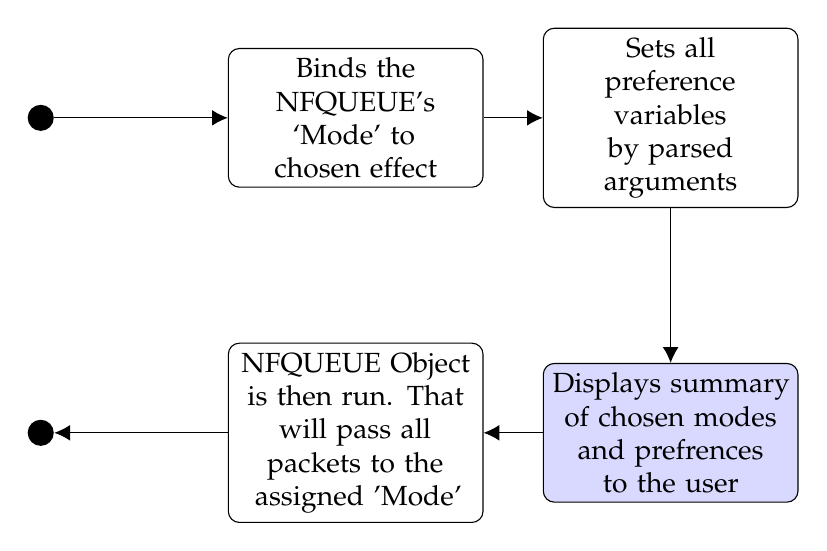
\begin{tikzpicture}

	\node (start) [shape=circle, fill=black]{};
	
	\node (setQueue) [right of=start, normal, xshift=\width]
	{Binds the NFQUEUE's `Mode' to chosen effect};
	
	\node (setVariables) [right of=setQueue, normal, xshift=\width]
	{Sets all \\ preference \\ variables by parsed \\ arguments};
	
	\node (userOutput) [fill=blue!15, below of=setVariables, normal, yshift=-\width]
	{Displays summary of chosen modes and prefrences to the user};
	
	\node (runNfqueue) [left of=userOutput, normal, xshift=-\width]
	{NFQUEUE Object is then run. That will pass all packets to the assigned 'Mode'};

	\node (end) [shape=circle, fill=black, below of=start, yshift=-\width]{};

	%Arrows
	\draw[->] (start)--(setQueue);
	\draw[->] (setQueue)--(setVariables);
	\draw[->] (setVariables)--(userOutput);
	\draw[->] (userOutput)--(runNfqueue);
	\draw[->] (runNfqueue)--(end);

\end{tikzpicture}
	\begin{figure}[h]
		\caption{UML Activity Diagram for assigning the choice of effect}
	\end{figure}
\end{center}


Choosing a mode for the program gives the ability to switch between degradation effect and arrangement of effects. This process is exactly the same for GUI and CLI. This is due to the shared code between the different user interfaces, all the CLI does is add a wrapper on top that allows control of the concealed code by the way of parsed arguments and the GUI just directly calls these methods when buttons are clicked.

\subsection{Incoming Packets}
\begin{center}
	\begin{tikzpicture}

	\node (start) [shape=circle, fill=black]{};
	
	\node (handler) [normal, right of=start, xshift=\width * 2] 
	{Packet placed into queue caught by handler method};
	
	\node (filterSet) [below of=handler, yshift=-\width, decision] {Is packet filter set?};
	\node (targetCheck) [left of=filterSet, xshift=-\width * 2, normal]{Check filter against packet};
	\node (passFilter) [below of=targetCheck, yshift=-\width, decision]{Does packet pass filter};
	
	\node (runEffect) [below of=filterSet, yshift=-\width, normal, fill=red!15]
	{Run assigned \\ effect on packet};	
	
	\node (Accept) 	[fill=blue!15, below of=passFilter, normal, yshift=-\width]{Accept Packet};
	\node (Drop)	[fill=blue!15, below of=runEffect, normal, yshift=-\width]{Drop Packet};	
	
	%Find the middle between the two nodes
 	\coordinate (CENTER) at ($(Accept)!0.5!(Drop)$);		
	\node (end)	[below of=CENTER, shape=circle, fill=black, yshift=-2cm]{};	
	
	\node (endLabel) [below of=end]{Thread released};	
	
	% Connections
	\draw[->] (start)--(handler);
	\draw[->] (handler)--(filterSet);
	
	\draw[->] (filterSet)--node[fill=white]{Yes}(targetCheck);
	\draw[->] (filterSet)--node[fill=white]{No}(runEffect);
	
	\draw[->] (targetCheck)--(passFilter);
	
	\draw[->] (passFilter)--node[fill=white]{Yes}(runEffect);
	\draw[->] (passFilter)--node[fill=white]{No}(Accept);	

	\draw[->] (runEffect)--(Accept);
	\draw[->] (runEffect)--(Drop);
	
	\draw[->] (Drop)--(end);
	\draw[->] (Accept)--(end);	
s
\end{tikzpicture}
	\begin{figure}[h]
		\caption{Activity diagram for running an effect on a single packet}
	\end{figure}
\end{center}

Above is the activity diagram for the process of running an effect on a single packet. The script automatically effects every packet that is placed in the NFQUEUE, this means protocol support does not need to be managed and no code manipulating or monitoring sockets is required.

% Section Description:
%
\section{Tool Class Design}
\subsection{Effect Class Diagram}

\begin{center}
	\begin{tikzpicture}

% Effect - Parent class
\umlclass{Effect}
{
	+ allow\_print 		: bool \\ 
	+ accept\_packets 	: bool
}
{
	+ print()			: void \\
	+ print\_stats()	: void \\
	+ effect()			: void 	
}

\umlclass[below right= 2cm of Effect]{Latency}
{
	+ latency\_value\_ms : int
}

\umlclass[below = 1.45cm of Effect]{PacketLoss}
{
	+ packet\_loss : int
}

\umlclass[below left= 2cm of Effect]{Bandwidth}
{
	+ rate\_limit : int
}

% Links
\umlVHVinherit{Effect}{Latency}
\umlVHVinherit{Effect}{PacketLoss}
\umlVHVinherit{Effect}{Bandwidth}

\end{tikzpicture}
	\begin{figure}[h]
		\caption{UML Class diagram for producing degradation effects}
	\end{figure}
\end{center}

The above design is for the various effects that will be implemented into the program. They will be self contained within separate modules encased in an object. This was chosen so each effect is modular and self contained from one another, this will improve the potential readability and maintainability of the code base, it will also make the code base much more scalable where effects can be added with high speed because of the lack of repeated code.  Each effect will inherit from the base class ``Effect", where it will obtain method and properties used for functionality, boolean variables for allowing printing and accepting packets, these are both necessary when `chaining' effects together, where a packet can only be accepted once and only a single print will be required.

\subsection{Effect Activity Diagram}
\begin{center}
	\includegraphics[scale=0.6]{Packet_Activity_Diagram}
	\begin{figure}[h]
		\caption{Activity Diagram for the degradation script}
	\end{figure}
\end{center}

Above is the activity diagram for the packet script that will implement the effect classes above, this script will be utilised directly from the command line or run by the GUI. The decision of having a single script that is controlled by multiple ways allow for one central point of functionality and means code can be shared throughout the project. The activity diagram shows the design choices for the direct control on the script. SIGINT is mentioned in the centre of the diagram, SIGINT is a built in signal in the Linux operating system that represents an interrupt signal, where it is triggered by pressing ``Control + C", this is the most common/clean way of stopping a script. The other alternatives to closing the script ``Control + Z" (SIGTSTP) and ``Control + /" (SIGQUIT) will be remapped to send a SIGINT signal and perform the same role, this will mean the program has one tidy point of closure.




% Section Description:
%
\section{Tool UI Design}
One of the ways mentioned before to control the degradation effects is by a user interface. It needs to have a way to easily add new buttons and text entries that link up to parameters in the script to make the interface scalable and easy to maintain, it also needs a window to display the same output as the terminal window, this can be achieved by `piping' the stdout to a custom section of the user interface. The `stdout' is the data stream that links up to a Linux terminal window, if the stdout points to somewhere else it will display where it is needed. Below is the initial drafted design for the user interface.

\begin{center}
	\includegraphics[scale=0.5]{Packet_UI_Design}
	\begin{figure}[h]
		\caption{Initial user interface design for the Degradation GUI}
	\end{figure}
\end{center}



% Section Description:
%
\section{Tool Implementation}

\subsection{NFQUEUE}
The script utilises a section in the Linux kernel referred to as the ``NFQUEUE". This is as the name suggests a queue that is stored in kernel memory that will store up packets until the user provides one of the two verdicts: `Drop' or `Accept'. The packets are pushed into this queue by the use of `iptable' rules, iptabales is a tool designed to filter packets by criteria. Below is a flow diagram for the path a packet might take, each table can have filtering rules embedded into to it:

% Diagram
\input{diagrams/iptables}

If there was a case where all packets entering the machine need filtering, an iptable rule would be added to the "Pre-Routing" section of the table to catch all packets entering the machine. 

So for example to move all packets entering from the network card into the NFQUEUE the iptable rule would be added like so:
\begin{center}
	\begin{console_font}
		\large{iptables -A INPUT -j NFQUEUE}
	\end{console_font} 
\end{center}
Where `-a' tells to append a rule onto the `INPUT' table and `-j' is the rule that affects the packet, in this case pushing it into the default queue.

This forms the main component of the functionality of the script, a series of iptable rules that filter packets into the NFQUEUE and allow to script to perform verdicts on each packet separately allows for effects to be easily applied to packets entering and leaving the machine.

Below is code for the creation of the NFQUEUE object along side the iptable rules:
\begin{Code}[]{NFQUEUE}
# iptables
os.system("iptables -A INPUT -j NFQUEUE")
os.system("iptables -A OUTPUT -j NFQUEUE")

# Setup for the NQUEUE
nfqueue = NetfilterQueue()

try:
	nfqueue.bind(0, mode)  # 0 is the default NFQUEUE
except OSError:
	print_force("[!] Queue already created")
	
nfqueue.run()
\end{Code}

In the code above the variable {\code mode} contains a method that performs effects on the packets. An example below shows what {\code mode} would equal if the effect chosen was latency:

\begin{Code}{Latency Packet Mode}
def packet_latency(packet):
    """This function is used to incur latency on packets"""
    if affect_packet(packet):
        assign_thread(latency_obj.effect, [[packet, time.time()]])
    else:
        packet.accept()
\end{Code}

There are a couple of aspect to note in the above code listing:
{\code affect\_packet} is the method that checks the packet against the active filters. {\code assign\_thread} is the method that assigns the object effect method ({\code latency\_obj.effect}) to an idle thread in the pool and 
{\code packet.accept()} and {\code packet.drop()} are the ways the packet is assigned a verdict, this can be done at any point in the code and becomes instantly active.


\subsection{Degradation Effects}
The script contains the functionality to simulate a plethora of effects and each effects functionality will be described below. Please not any of these effects can be chained together in any order.

\subsubsection{Latency}
Latency as described in the background section is the delay in initiating a task and seeing its results. Latency is simulated by using a timing mechanisms where the arrival time of the packet is saved. The packet is then pushed into the NFQUEUE that triggers a single thread that will hold the packet for a set amount of time, the holding time is calculated by taking the amount of time the packet has already been in the script away from the target time. The packet is then marked as `ACCEPTED' and pushed out of the queue.

\begin{Code}{Latency}
def custom_effect(self, packet):
	"""Thread functionality"""

	# # Dynamic time mode
	# Parameters contained within a single object
	if type(packet) is list:
		packetObj = packet[0]
		startTime = packet[1]

		# Works out the time difference between
		# thread conception and now
		elapsed = time.time() - startTime
            
		# Take the elapsed time off the target
		wait_time = self.latency_value - elapsed

		if wait_time < 0:
			pass
		else:
			time.sleep(wait_time)
			self.accept(packetObj)
			
		# # Static time mode
		else:
			time.sleep(self.latency_value)
			self.accept(packet)

\end{Code}

\subsubsection{Packet Loss}
Packet loss is simulated by first assigning a target value, lets say for this example 10\%. For each packet the script randomly generates a number between 1 and 100, if that value is less than the target value the packet is dropped, and if the value is larger the packet is accepted. This therefore creates the effect of packet loss. It does however require a fair amount of packets to balance out statistically and reach the percentage target.

\begin{Code}{Packet Loss}
def custom_effect(self, packet):
        """This function will issue packet loss,
           a percentage is defined and anything
           lower is dropped and anything higher is accepted"""

        if self.packet_loss_percentage != 0:

            # random value from 0 to 100
            random_value = random.uniform(0, 100)

            if self.packet_loss_percentage > random_value:
                self.dropped_packets += 1
                packet.drop()

            # Accept the packet
            else:
                self.accept(packet)
        else:
            self.accept(packet)
\end{Code}

\subsubsection{Bandwidth}
There are two modes created for bandwidth; rate limiting and a simple display. Rate limiting allows the script to limit the rate of bandwidth flowing through the machine and calculates the rate transferred over a period of 5 seconds, if the rate is higher it waits until the rate drops below the target. This gives it the ability to adjust quickly and allows the script to be run for a long period of time without the overall average of the bandwidth affecting future changes. Displaying the bandwidth work exactly the same but without the limit check, this is useful when checking the current download speeds or the max transfer rate.

Limiting bandwidth is below:

\begin{Code}{Bandwidth Limit}
def custom_effect(self, packet):
	"""Used to limit the bandwidth"""

	# Adds packet to the backlog
	self.packet_backlog.append(packet)
	
	# The algorithm will send until the backlog is empty or 
	# the limit is exceeded
	while self.rate < self.bandwidth and len(self.packet_backlog) > 0:
		self.send_packet(self.packet_backlog[0])
            
		# Packet is removed from the list
		del self.packet_backlog[0]
			
		self.calculate_rate_overall_avg()
\end{Code}

\subsubsection{Out-of-order}
This effect changes the order of packets coming into the script, this can be used to check its effect on UDP and TCP and can test how quickly these issue can be rectified. It works by queuing up every packet into a list, then a single thread randomly picks an index of that list, accepts the packet and allows it to leave. This therefore means at its most extreme the order can be last in, first out.

\subsubsection{Connection Simulation}
Connection simulation isn't quite a degradation effect but its intent is to simulate the effect of degradation on a common connection like `WiFi` or a 3G connection to see how these are effected by said degradation. This can be useful in some situations where for example testing a mobile applications performance over 3G with heavy latency, the mobile would connect to the script and the script would effect any traffic entering or leaving the handset.

\subsubsection{Jitter}
Jitter mode clumps and separates packets in their transmission, with some it waits a small period of time other it will clump up delay as a total and then send them all at once. This is to test how the protocol deals with jitter in the connection. Jitter as explained in the background is the intra-packet latency i.e. the difference in time between arrivals of packets.

\subsection{ARP Spoofing}
The script also supports an ARP spoofing mode that allows it to sit between a gateway and a specified target. This means the script can perform all its functions on a single target with a very quick deployment time. As touched on in the background the ARP protocol performs no authentication on any changes to the ARP cache meaning that you can perform a man in the middle attack and route traffic through a machine of your choice.

The script begins by grabbing the MAC addresses connected to the provided gateway and target IP addresses. Two ARP reply packets (denote by the `2' opcode) are sent out: One telling the victim that the current machines MAC address maps to the gateway, and the other telling the gateway that the victims IP maps to the current machines MAC address.

Below is the process visualised:

\newcommand{\cisco}{cisco_images}
\newcommand{\scale}{0.7}

% Gateway
\newcommand{\GatewayLabel}{
\begin{tabular}{l l}
Gateway\\
\hline
\vspace{0.1cm}
\bf{192.168.1.1} & \bf{C8:49:BD:82:47:4D}\\
ARP Cache\\
\hline
192.168.1.2 & 46:41:73:EC:70:E3
\end{tabular}
}

%Victim
\newcommand{\VictimLabel}{
\begin{tabular}{l l}
Victim\\
\hline
\vspace{0.1cm}
\bf{192.168.1.2} & \bf{46:41:73:EC:70:E3}\\
ARP Cache\\
\hline
192.168.1.1 & C8:49:BD:82:47:4D
\end{tabular}
}

\begin{center}
\begin{tikzpicture}[
    diagram item/.style={},
    align=left
]         

\node (Router)[
    diagram item,
    label=above:\GatewayLabel,
    yshift=-2cm
] {\includegraphics[scale=\scale]{\cisco/router}};

\node (Victim)[
	diagram item,
	label=above:\VictimLabel,
	right of=Router,
	xshift=7cm
] {\includegraphics[scale=\scale]{\cisco/workstation}};


\draw[-] (Router)--(Victim);

\end{tikzpicture} 
\end{center}


As you can see both ends are connected and have gone through the process to resolve the IP addresses to MAC addresses, you can see above each device their corresponding IP, MAC and ARP Cache. The ARP cache as mentioned previously is a record linking IP addresses to MAC addresses.

\newcommand{\tgap}{0.1cm}

% Gateway
\newcommand{\GatewayLabelAfter}{
\begin{tabular}{l l}
Gateway\\
\hline
\vspace{\tgap}
\bf{192.168.1.1} & \bf{C8:49:BD:82:47:4D}\\
ARP Cache\\
\hline
192.168.1.2 & \bf{\textcolor{red}{37:A8:22:F6:BB:34}} \\
192.168.1.3 & 37:A8:22:F6:BB:34
\end{tabular}
}

%Victim
\newcommand{\VictimLabelAfter}{
\begin{tabular}{l l}
Victim\\
\hline
\vspace{\tgap}
\bf{192.168.1.2} & \bf{46:41:73:EC:70:E3}\\
ARP Cache\\
\hline
192.168.1.1 & \bf{\textcolor{red}{37:A8:22:F6:BB:34}} \\
192.168.1.3 & 37:A8:22:F6:BB:34
\end{tabular}
}

%Attacker
\newcommand{\AttackerLabel}{
\begin{tabular}{l l}
Attacker\\
\hline
\bf{192.168.1.3} & \bf{37:A8:22:F6:BB:34} 
\end{tabular}
}

\begin{center}
\begin{tikzpicture}[
    diagram item/.style={},
    align=left
]         

\node (Router)[
    diagram item,
    label=above:\GatewayLabelAfter,
    yshift=-2cm
] {\includegraphics[scale=\ciscoImageScale]{\cisco/router}};

\node (Victim)[
	diagram item,
	label=above:\VictimLabelAfter,
	right of=Router,
	xshift=7cm
] {\includegraphics[scale=\ciscoImageScale]{\cisco/workstation}};


%Find the middle between the two nodes
\coordinate (CENTER) at ($(Victim)!0.5!(Router)$);		
\node (Attacker)[
	label=below:\AttackerLabel,
	below of=CENTER,
	yshift=-3.5cm
] {\includegraphics[scale=\ciscoImageScale]{\cisco/laptop}};

\draw[red, very thick] (Router)--(Attacker);
\draw[red, very thick] (Attacker)--(Victim);


\end{tikzpicture} 
\end{center}


Note after the 3rd device connects to the network, both devices gain a record of its IP and MAC address in their ARP cache. 

After both spoofed packets have been send out the ARP cache for each receiving end gets updated, the text in red shows the changes caused by the spoofed ARP packets. Now when either end wants to talk to each other it will resolve the MAC address and send it with the new MAC address in the table, this will therefore get routed through the attacking PC and will allow the script to receive all the traffic between the two parties.

\subsection{Network Attacks}
A couple of network attacks were implemented into the script, these served the purpose of providing very heavy artificial traffic designed to create heavy loads or mess with integral protocols. Not many attacks were added as they don't provide much purpose apart from stress testing and they reside on the edge of the scope of this project. There will also be a brief discussion into possible techniques to mitigate the effects. 

\subsubsection{UDP Flooding}
UDP flooding is a very simple attack, lots of UDP packets are created and send over a network stream very quickly. This attack is designed to `flood' the buffers in the receiving machine and slow down or event prevent internet connection. The script creates 10 or so threads that create and send packet concurrently, this amount of threads easily reaches the max throughput of the test machines NIC card and massively reduces internet connection on the receiving end.

The attack could be detected and prevented by a script that monitors the network transfers rates, this attack will create a huge spike in the transfer rate that can be detected and all traffic would be blocked from the sending party.

\subsubsection{ARP Spamming}
This attack works by once again exploiting the lack of authentication of the ARP protocol. In the entire network mode the script starts by detecting all active hosts on a network, it then starts sending out falsified ARP reply packets with randomly generated MAC addresses inside. This results in all computers on the networking having incorrect ARP cache values and resulting in computers incorrectly resolving IP and MAC address combinations and traffic not being allowed through.

This attack is relatively easy to execute but can simply be prevented by issuing static ARP tables for each machine, this prevents unsolicited ARP replies from changing IP and MAC address combinations and also prevents ARP Spoofing from occurring on that network.


%Experimental design:
%If you project includes any experiments, including but not limited to user testing, then you can discuss their design here. Note that again this does not exist in a vacuum and should be tied to your research.

\section{Test design and system testing}
There are various sections of the project that require a separate testing plan:

\begin{itemize}

	\item Traffic simulation programs\\
	These are the client server programs that will simulate traffic over the synthetic net. These tests will need to 	make 	sure each client and server performs its role correctly.
	
	\item Packet script and effects\\
	This is the script that will run on the custom router. Tests will be checking effects do their basic jobs and the script can be controlled effectively.
	
\end{itemize}

\subsection{Traffic simulation programs}
The test plan for this section will need to check all the intended functionality of each window. There are three aspects of each that will need testing:

\begin{itemize}

	\item UI \\
	Tests will be created that click buttons and check the user interface works effectively through automated testing.

	\item Business Logic \\
	Code behind the UI will have the relevant methods testing with expected and actual results.

	\item Real world usage \\
	The involvement of multiple windows and more complex functionality can be tested by using automated testing 			scripts.
	
\end{itemize}

Appendix A contains the test plan for the program, each separate program has had its user interface and business logic tested and programs that are to be used together have had ``Live" tests created to check their interaction together. The automated tests have been achieved by using the CUIT (Coded User Interface Tests) \footnote{\url{https://msdn.microsoft.com/en-us/library/dd286726.aspx}} that are built into Visual Studio 2017. These allow clicks and movements to be recorded and repeated.

\subsection{Packet Script}
It was decided that a separate test plan was needed for the script that will be run on the router. This was because its design is considerably different to that of the traffic simulation programs. Each individual effect needs a basic test that uses a loopback ping test to simulate incoming traffic where a criteria is looked for, for example to test packet loss, the test pings the script until a packet is lost or a time-out is reached, this can perform a basic test on the functionality of the effect. Each effect will also require validation for the passed parameters, there will be a test created that will test various values inside and outside of the validation range.

\subsection{Testing methodology considerations}
Initially the methodology chosen to start development of the traffic simulation programs was ``Test Driven Development" \citep{beck2003test}, this was a tight methodology that increased development time and gave the added benefit of showing that new changes have not broken older functionality. This methodology was good to start off the project and allowed for a tight structure to be created where no time was wasted debugging previously working code, but as mentioned this methodology slowed development time down, this was chosen to be abandoned after 3-4 weeks to an ad-hoc approach. 
This change was due to time restraints on the project and the less-important role that the traffic simulation programs had on the project compared to the degradation simulation script. The degradation script was developed in the ad-hoc approach, this was due to issue stated previously about the unknown aspects of the script and how it would be operating that it was decided that the time invested to write up test scripts would assume too much and would risk them having the be completely rewritten, tests therefore was added alongside new functionality.





% Section Description
%
\section{Experiential design}
\subsection{Latency Accuracy}
In the initial stages of the project there were experiments that tested the effects of the degradation on the network, the tests were performed on the loopback (Internal network 127.0.0.1) with ICMP ping packets.

This test was designed to show the accuracy of different ways of simulating latency, the first way being a static timer that just causes the thread to sleep for a set amount of time or a dynamic timer that calculates the elapsed time since the creation of the thread and the command telling the thread to sleep, the dynamic timer takes this elapsed time off the target latency value.

Below the results are visualised in a single graph. Please note - the relatively high percentage error in the small ranges of latency this is due to the error proportion being a much larger chunk of the overall target latency and therefore being a higher percentage error:

\begin{tikzpicture}[every axis plot/.append style={thick}]
		\begin{axis}[
			width=\linewidth,
			height=10cm,
			grid=major,
			xmin=1, xmax=100,
			ymin=0, ymax=100,
			xlabel=Latency (ms),
			ylabel=Error (\%)]
			\addplot table [x index=0, y index=1, mark=none, search path=csv_data, col sep=comma]{PingTestDynamicVsStatic.csv};		
			\addlegendentry{Static}	
			
			\addplot table [x index=0, y index=2, mark=none, search path=csv_data, col sep=comma]{PingTestDynamicVsStatic.csv};		
			\addlegendentry{Dynamic}	
		 \end{axis}
 \end{tikzpicture}
 

As you can see from the graph the dynamic form of issuing latency is overall more accurate in simulation, but however, it is still not perfect and there seems to be a small overall error present. This performance is however more than suitable for the scope of this project.

\subsection{Visualising effects}
The most effective way to visualise real world connections were running tests on SpeedTest.net \footnote{\url{http://beta.speedtest.net/}}. This is very useful to quickly visualise a certain effect on the network.

Below are two images showing the effect of a 100ms latency on a networks speed. Both tests were performed on the same empty network and the best result was taken from 5 runs on each.

\begin{center}
	\includegraphics[scale=0.5]{SpeedNoEffect}
	\begin{figure}[h]
		\caption{The initial connection speed}
	\end{figure}
\end{center}

\begin{center}
	\includegraphics[scale=0.5]{Speed100ms}
	\begin{figure}[h]
		\caption{Network speed with a latency of 100m/s}
	\end{figure}
\end{center}

As you can see from both images, the 100ms has evidently been applied effectively and the speed of the connection has dropped by around 10Mbps. This means in real world terms the time taken to download a 1GB file would take 35 seconds longer to download. This is not a considerable reduction but the latency is having a obvious effect on the network quality.
	%In this chapter you must evaluate your overall project achievement, and provide a clear statement of where the delivered results stand in relation to the original project goals. You should also provide an outline of any further potential work which you can foresee as beneficial to the future development of your project.
\chapter{Evaluation}


%The tool is used to create results and there're discussed here
\section{Experimentation Results}

	\subsection{Effect of Packet Loss on Download Speeds}
	\subsubsection{Packet Loss and its effect on download speeds}

% Better graph needed
\begin{center}
	\includegraphics[scale=0.6]{PL_Download}
	\begin{figure}[h]
	 	\caption{Graph displaying effect of packet loss on download speeds}
	\end{figure}		
\end{center}






The graph above shows the download speed measured in Mbps against the increasing rate of packet loss, as you can see the download rate only reaches around 25\%, this is due to the connection test failing at anything above. The tests were performed by using Iperf on the localhost as to reduce any degradation that may exists already in an existing network.

My initial hypothesis for the sharp decreases in packet loss from 0\% to 1\% is due to the congestion control mechanisms built into TCP. TCP as mentioned in the background section allows for multiple devices to co-exist on a network and needs to dynamically balance network resources for every client, it performs this through congestion control algorithms where packet loss in this aspect is assumed as a sign of congestion to the algorithm where it adapts by reducing its transfer rate each time a packet is lost, this means the transfer rate drastically reduces until it reaches a platform. The transfer rate is dictated by a few factors, one known as the congestion window (Cwnd) and the advertised size of the receiving window (Rwnd). The overall window size is the smaller of these two numbers, and the smaller the window size, the less packets can be send in one time frame. The congestion window therefore is reduces every time packet loss is detected. 

The test devised to prove this hypothesis will involve once again an iperf client/server where a packet is dropped after a time period while the congestion window size is tracked. Below is a graph showing the result of a test spanning 10 seconds where a single incoming packet was dropped every 1 second, the graph is measuring Cwnd sizes on the y axis and Time on the x axis.

%Graph
\begin{center}
	\begin{tikzpicture}[]
		\begin{axis}[
			width=\linewidth,
			height=10cm, 
			grid=major,
			xlabel=Time,
			ylabel=Cwnd]
			\addplot table [mark=*, search path=csv_data, col sep=comma]{PacketLossCwnd.csv};
			
		 \end{axis}
 	\end{tikzpicture}
\end{center}

As you can see around the 1 second mark there are almost identical drops in the Cwnd size, this demonstrates that packet loss causes the congestion window to reduce in size and if packet loss is substantial enough can cause a huge drop in transfer rates.

Please also note the initial increase in transfer rate, this is displayed in the graph below:

\begin{center}
	\includegraphics[scale=0.6]{TCP_Slow_Start}
	\begin{figure}[h]
	 	\caption{Close up of the initial start}
	\end{figure}		
\end{center}

This is known as the TCP Slow start and this is used by the protocol to naturally align itself into the network eco-system, it starts off with a modest transfer rate to prevent situations where an initial abnormally large transfer rate would fill buffers and cause network congestion and adjusts by incorporating the techniques explained above to manually adjust its transfer rate to fit naturally into the current network.
 

	%TODO - Comparason between congestion algos 
	%			- Reno
	%			- Cubic

%Project Achievements:
%You should consider your original goals and statewh clearly ich have or have not been fully or partially met, and discuss reasons for any significant variance.
\clearpage
\section{Project Achievements}

{\bf Initial Goal}\\
{\it Create a custom simulated network that can demonstrate and visualise network degradation and common DoS attacks, this is so network engineers can identify weak spots and points of strain}

% URLS
\newcommand{\chromeUrl}{\url{https://www.google.com/chrome/index.html}}
\newcommand{\firefoxUrl}{\url{https://www.mozilla.org/en-US/firefox/new/}}
\newcommand{\fileZillaUrl}{\url{https://filezilla-project.org/}}

\subsection{Objective One}
{\it Develop a fully working clients and servers that communicate using HTTP/1.1 and FTP over the TCP protocol alongside a client and server that use the UDP protocol}

This objective initially involved the creation of custom client server solution for HTTP, FTP and UDP. This involved a lengthy development period where each client and server would require the implementation of required features for the project. It was decided after a period of 3.5 weeks that the simulated network having a custom solution created no added value to the initial goal of the project, this is why HTTP has been replaced by pre-existing browsers such as Google Chrome \footnote{\chromeUrl} or Mozilla Firefox \footnote{\firefoxUrl} and and FTP solution replaced by FileZilla's \footnote{\fileZillaUrl} server and client pair. These are all projects that have had multiple years invested into their development and offer increased stability and selection of features with next to zero investment in time development time for this project and they have all the features required to meet the goal of this project. UDP on the other hand was left as a custom solution, for the sacrifice of realism the UDP client and server show a easy to view visualisation of UDP packet loss and is very effective at what it does.

However, even with the changes each sub point of the object has been met.

\subsection{Objective Two}
{\it Create a program that runs on a Linux based OS that can be used to simulate degradation and attacks. This program will then be run on the router.}

In the aims and objectives section lists out the criteria required to meet this objective. The created solution meets all of these criteria. It provides the functionality to simulate packet loss, latency and bandwidth plus a selection of other effects. The other effects were chosen to provide more depth to the project and allow the possibility to chain effects together to simulate more sophisticated degradation. The script also allows UDP flooding and ARP spamming. It contains a mode to increment the TTL but this mode was discarded from the main advertised functionality due to its inherit difficulty in displaying its effect on a connection due to the hard task for forming loops in a networks structure. This script is also functional on the set-up Raspberry Pi Router.


\subsection{Objective Three}
{\it Create a working custom router that can be used to simulate degradation in conjunction with the program outlined in Objective 2}

The project has met the requirements of this objective. The router can be used in place of a commercial router and can handle around 3 clients at a single time while still providing acceptable transfer speeds. A client can connect to the router by wireless or wired means.

\subsection{Overall}
%TODO - Explain how the overall goal has been met

%Further work:
%You should identify any specific areas of the existing product where further work is required, either to address known bugs or omissions, or to improve the system – for example an area you developed at an early stage may in hindsight have been structured in a better way, although it is still perfectly functional.
%You should also provide an outline of any additional areas of potential development you can envisage beyond the initial goals, where the system might be extended in future for greater functionality.
\section{Further work}
	\chapter{Conclusion}
%The conclusion to your project should contain a summary of your project as you documented it in the preceding text.
%It should be clear and concise and include the main contributions of the project.
%It often works well to have the conclusion be a matching bookend for the introduction and aims of your project.

The project as mentioned above has succeeded in achieving its goals, it was able to provide a test network where various forms of degradation were performed on the network using a script hosted on a small Raspberry Pi router. The script is supported by a Linux OS and performs most of its functionality utilising a section in the Linux Kernel known as the NFQUEUE. Although further improvements were discussed above the project was fully functional and the tool can be used to simulate degradation very effectively.
	\begin{appendices}

%
\chapter{Test Plan}
\label{ref:testplan}
\small
\begin{longtable}{| p{1.5cm} | p{1.5cm} | p{3cm} | p{4cm} | p{3cm} |}
	\hline
		%HEADER
		\bf{Section} & \bf{Test Code} & \bf{Test Name} & \bf{Description} & \bf{Expected} \\ \hline
		
		%--- UDP CLIENT
		\bf{UDP Client}&&&& \\ \hline
		
		% Business Logic
		Logic &&&& \\ \hline
		&UC-L1& TestStartUp() & Creates a client object before each test & n/a\\ \hline
		&UC-L2& TestCleanUp() & No clean-up needed & n/a \\ \hline
		&UC-L3& Connect-Disconnect() & The client connects performs no action then disconnects & n/a \\ \hline
		&UC-L4& CreateClientObj() & A client object is created & n/a \\ \hline
		&UC-L5& SendPacket() & Sends a single UDP packet & n/a\\ \hline
		&UC-L6& CheckGridSend() & Checks the method sends out the correct number this depends on grid size & n/a \\ \hline
		
		% UI
		UI &&&& \\ \hline
		&UC-U1& TestStartUp() & Loads up a fresh window from the command line & n/a \\ \hline
		&UC-U2& TestCleanUp() & Clicks the X in the top right corner & n/a \\ \hline
		&UC-U3& ConnectClick() & Clicks the "Connect" button & n/a \\ \hline
		&UC-U4& RestartClick() & Clicks the "Connect" button then the "Restart" button & n/a \\ \hline
		&UC-U5& Connect-InvertCheck() & Clicks the "Connect" button and checks all the buttons invert their "Enabled" property correctly & Connect(Disabled), Restart(Enabled) \\\hline
		&UC-U6& Restart-InvertCheck() & Clicks the "Connect" button, then the "Reset" button and checks the "Enabled" properties for all buttons are correct & Connect(Enabled), Restart(Disabled) \\\hline
		&UC-U7& TextEntry() & Enters text into the text box and then "Connect" is clicked & n/a \\ \hline
				
		%--- UDP SERVER
		\bf{UDP Server} &&&& \\ \hline		
		
		%Business 
		Logic &&&& \\ \hline
		&US-L1& TestStartUp() & Creates the client object & n/a \\ \hline
		&US-L2& TestCleanUp() & n/a & n/a  \\ \hline
		&US-L3& CreateObject() & Tests that the server object can be created successfully & n/a \\ \hline
		&US-L4& WaitForTimeout() & Starts the server and checks it closes cleanly after time-out & n/a \\ \hline
		
		% UI
		UI &&&& \\ \hline
		&US-U1& TestStartUp() & 
		Loads up a fresh window from the CMD line & n/a \\ \hline

		&US-U2& TestCleanUp() & 
		Clicks the X in the top right hand corner & n/a  \\ \hline
		
		&US-U3& StartClick() & Click the "Start" button & n/a \\ \hline
		&US-U4& RandomiseClick() & Click the "Randomise" button & n/a \\ \hline
		&US-U5& Start-ResetClick() & Clicks the "Start" button then resets and checks it returns to it's default state & n/a \\ \hline
		&US-U6& Randomise-ResetClick() & Clicks the "Randomise" button, the resets and checks it returns to it's default state & n/a \\ \hline
		&US-U7& Start-CheckInvert() & "Start" button clicked and then the test checks for "Enabled" property is inverted & n/a \\ \hline
		&US-U8& RestartCheckInvert() & "Start" then "Restart" button clicked and the test then checks for the correct inverting of the buttons "Enabled" property Start = Enabled, Restart = Disabled & n/a \\ \hline
		&US-U9& Stat-PacketLossReset() & Checks when the restart button is clicked the statistics is returned to default & "-" \\ \hline
		&US-U10& Stat-TotalPacketLossReset() & Checks when the restart button is clicked the statistics is returned to default & "-" \\ \hline
		&US-U11& Stat-TotalPacketSentReset() & Checks when the restart button is clicked the statistics is returned to default & "-" \\ \hline
		&US-U12& Stat-CheckDeafult() & "Start" is clicked and the test then waits for a time-out, it then checks the default values of the statistics & PacketLoss(100) \\ \hline
		
		%--- UDP COMBINED		
		Live Tests &&&& \\ \hline
		&U-1& TestStartUp() & Both windows were opened on the command line & n/a \\ \hline
		&U-2& TestCleanUp() & Both windows are closed by automated actions & n/a \\ \hline
		&U-3& SendAndRecieve-Valid() & The client sends packages to the server and the server accepts packets & n/a \\ \hline
		&U-4& SendAndRecive-Valid-Twice() & The performs the same action at the above test but does the whole loop an extra time to check if the reset works correctly & n/a \\ \hline
		&U-5& SendAndRecieve-Invalid() & This test doesn't connect the client to the server but a random IP on the network, this is to check the server will act accordingly & n/a \\ \hline
\end{longtable}

Packet Script Test Plan for the default effects.

\begin{longtable}{| p{1.5cm} | p{1.5cm} | p{3cm} | p{4cm} | p{3cm} |}
	\hline	
	\bf{Section} & \bf{Test No} & \bf{Test Name} & \bf{Description} & \bf{Expected} \\ \hline
	\bf{Effects} &&&& \\ \hline
	
	% -- 	
	PacketLoss &&&& \\ \hline
	&P-1	& StartPacketLoss() 
	& Starts the script with the expected parameter (e.g. -pl 10) &  Script should start PacketLoss mode \\ \hline
	
	&P-1	& PacketLossEffect() 
	& Pings the script and checks the effect on the ping packets, the test pings until one packet is lost. Checking for exact percentages isn't reliable enough & Some packet loss \\ \hline	
	
	% -- 	
	Latency &&&& \\ \hline
	&L-1& StartLatency() 	& Starts the script with valid parameters for latency (e.g. -l 10) & Script should start in Latency mode \\ \hline
	&L-2& LatencyEffect() 	& Pings the script and checks the latency value within a margin of error & Latency effect 		on ping packets \\ \hline
	
	% -- 
	Bandwidth &&&& \\\hline
	&B-1& StartBandwidth() &  Starts the script with the expected parameters (e.g. -rl 100) & Script should start in Bandwidth limit mode \\ \hline
	&B-2& BandwidthEffect() & Starts bandwidth mode and starts pinging the localhost, after a certain amount of packets the rate is calculated and checked against the rate limit value & n/a \\\hline
	
	Out-Of-Order &&&& \\\hline
	&O-1& StartOrder() & Starts the script and checks the effect initialises correctly & n/a \\\hline
	&O-2& OutOfOrderEffect() & Starts the effect and checks using the localhost that the packet sequence numbers are not in sequential order when they return & n/a \\\hline
	
	Jitter &&&& \\\hline
	&J-1& StartJitter() & Starts the script in the mode and checks all initialisation finishes correctly & n/a \\\hline
	&J-2& JitterEffect() & Ping packets are sent on the localhost and a difference in packet latency is looked for  & n/a\\\hline
	
	% -- 	
	Validation &&&& \\ \hline
	&V-1& LatencyValidation() & Check that the validation works for the latency mode & Range = 1-1000ms \\\hline
	&V-2& PacketLossValidation() & Check that the validation works for the packet loss mode & Range = 1-100\%\\\hline
	&V-3& BandwidthValidation() & Checks that validation works for bandwidth mode & Range = 1-10000B/s\\\hline
	&V-4& JitterValidation & Checks that validation works for difference values & Range = 10ms-100ms \\\hline	
	
\end{longtable}

%
\chapter{GitHub Issues}
\begin{center}
	\label{ref:GitHubAppendix}
	\includegraphics[scale=0.6]{github_issues}
	\begin{figure}[h]
		\caption{Snapshot of actual issues created in the project}
		\label{ref:GitHubIssues}
	\end{figure}			
\end{center}

\begin{center}
	\includegraphics[scale=0.6]{github_issue_des}
	\begin{figure}[h]
		\caption{Example of an issue with discussion}
		\label{ref:GitHubIssueExample}
	\end{figure}	
\end{center}

%
\chapter{Testing Correctness}
\begin{center}
	\label{ref:testingCorrect}
	\begin{tabular}{| p{3cm} | p{5cm} | p{1cm} |}
	
	\lineend
	%--- UDP CLIENT
	\header{UDP Client}\lineend
	
	\bf{Logic} && \\ \lineend
	UC-L3	& Connect-Disconnect() 			& \Pass \\ \lineend
	UC-L4	& CreateClientObj() 			& \Pass \\ \lineend
	UC-L5	& SendPacket() 					& \Pass \\ \lineend
	UC-L6	& CheckGridSend() 				& \Pass \\ \lineend
	
	\bf{UI} && \\ \lineend	
	UC-U3 	& ConnectClick() 				& \Pass \\ \lineend
	UC-U4	& RestartClick() 				& \Pass \\ \lineend
	UC-U5	& Connect-InvertCheck() 		& \Pass \\ \lineend
	UC-U6	& Restart-InvertCheck() 		& \Pass \\ \lineend
	UC-U7	& TextEntry() 					& \Pass \\ \lineend
	
	%--- UDP Server
	\header{UDP Server}\lineend
	
	\bf{Logic} && \\ \hline
	US-L3	& CreateObject() 				& \Pass \\ \lineend
	US-L4	& WaitForTimeout() 				& \Pass \\ \lineend	
	
	\bf{UI} && \\ \lineend
	US-U3	& StartClick()					& \Pass \\ \lineend
	US-U4	& RandomiseClick() 				& \Pass \\ \lineend
	US-U5	& Start-ResetClick() 			& \Pass \\ \lineend
	US-U6	& Randomise-ResetClick()		& \Pass \\ \lineend
	US-U7	& Start-CheckInvert() 			& \Pass \\ \lineend
	US-U8	& RestartCheckInvert() 			& \Pass \\ \lineend
	US-U9	& Stat-PacketLossReset()		& \Pass \\ \lineend
	US-U10	& Stat-TotalPacketLossReset() 	& \Pass \\ \lineend
	US-U11	& Stat-TotalPacketSentReset() 	& \Pass \\ \lineend
	US-U12	& Stat-CheckDeafult()		  	& \Pass \\ \lineend
		
	\header{UDP Combined}\lineend
	\bf{Live} && \\ \lineend
	U-3		& SendAndRecieve-Valid() 		& \Pass \\ \lineend
	U-4		& SendAndRecive-Valid-Twice() 	& \Pass \\ \lineend
	U-5		& SendAndRecieve-Invalid() 		& \Pass \\ \lineend	
	
\end{tabular}

	\begin{figure}[h]
		\caption{Testing correctness for the UDP Server and Client}
		\label{ref:testingUDP}
	\end{figure}
	
	\begin{tabular}{| p{3cm} | p{5cm} | p{1cm} |}

\lineend
\header{PacketLoss}
P-1		& StartPacketLoss() 		& \Pass \\ \lineend
P-2		& PacketLossEffect()		& \Pass \\ \lineend

\header{Latency} 
L-1		& StartLatency() 			& \Pass	\\ \lineend
L-2		& LatencyEffect() 			& \Pass \\ \lineend

\header{Bandwidth} 
B-1		& StartBandwidth()			& \Pass \\ \lineend	
B-2		& BandwidthEffect() 		& \Pass \\ \lineend

\header{Out-Of-Order}
O-1		& StartOrder()				& \Pass \\ \lineend
O-2		& OutOfOrderEffect()		& \Pass \\ \lineend

\header{Jitter}
J-1		& StartJitter()			 	& \Pass \\ \lineend
J-2		& JitterEffect() 			& \Pass \\ \lineend

\header{Validation} 
V-1		& LatencyValidation() 		& \Pass \\ \lineend
V-2		& PacketLossValidation() 	& \Pass \\ \lineend
V-3		& BandwidthValidation()	 	& \Pass \\ \lineend
V-4		& OutOfOrderValidation()	& N/A 	\\ \lineend
V-5		& JitterValidation()		& \Pass \\ \lineend
\end{tabular}
	
	\begin{figure}[h]
		\caption{Testing correctness for the main script functions}	
		\label{ref:testingScript}
	\end{figure}
\end{center}
\end{appendices}

	
	\bibliographystyle{hull}
	\bibliography{report}
	
\end{document}
